%%%%%
%%
%% Plan van Aanpak
%%
%% Version: v0.1
%% Authors: Iain Munro
%% Date: 18/02/2018
%%%%%

%Install packages using:
%sudo tlmgr install

% Available documentclass options:
%
%   <all `report` document class options, e.g.: `a5paper`>
%   withindex   - enables the index. New index entries can be added through `\index{my entry}`
%   glossary    - enables the glossary.
%   techreport  - typesets the thesis in the technical report format.
%   firstyr     - formats the document as a first-year report.
%   times       - uses the `Times` font.
%   backrefs    - add back references in the Bibliography section
%
% For more info see `README.md`
\documentclass[firstyr,a4paper,oneside]{cam-thesis}%withindex
\usepackage[dutch]{babel}
% Citations using numbers
\usepackage[numbers]{natbib}

\newcommand{\thesisTitle}{Allianz - Automatiseren Claim Process}

\usepackage[utf8]{inputenc}

%APA norm
\usepackage{babel} 
\usepackage{apalike}
\bibliographystyle{apalike}

%tables new lines
\usepackage{makecell}

%Set the title spacing correctly
\usepackage{titlesec}
\titlespacing{\chapter}{0pt}{0pt}{0pt}
\titlespacing{\section}{0pt}{0pt}{0pt}
\titlespacing{\subsection}{0pt}{0pt}{0pt}

%Om de pagina margins etc te debuggen
%\usepackage{showframe}

\usepackage{pgfgantt}
\usepackage{rotating}
\usepackage[graphicx]{realboxes}

%%%%%%%%%%%%%%%%%%%%%%%%%%%%%%%%%%%%%%%%%%%%%%%%%%%%%%%%%%%%%%%%%%%%%%%%%%%%%%%%
%% Style (Changing the visual style of chapter headings and stuff.)
%%
\RequirePackage{titlesec}
% [Fixes issue #34 (see https://github.com/cambridge/thesis/issues/34). Solution from: http://tex.stackexchange.com/questions/299969/titlesec-loss-of-section-numbering-with-the-new-update-2016-03-15
\RequirePackage{etoolbox}
\makeatletter
\patchcmd{\ttlh@hang}{\parindent\z@}{\parindent\z@\leavevmode}{}{}
\patchcmd{\ttlh@hang}{\noindent}{}{}{}
\makeatother
% end of issue #34 fix]
\newcommand{\PreContentTitleFormat}{\titleformat{\chapter}[display]{\scshape\Large}
{\Large\filleft\MakeUppercase{\chaptertitlename} \Huge\thechapter}
{1ex}
{}
[\vspace{1ex}\titlerule]}
\newcommand{\ContentTitleFormat}{\titleformat{\chapter}[display]{\scshape\huge}
{\Large\filleft\MakeUppercase{\chaptertitlename} \Huge\thechapter}
{1ex}
{\titlerule\vspace{1ex}\filright}
[\vspace{1ex}\titlerule]}
\newcommand{\PostContentTitleFormat}{\PreContentTitleFormat}
\PreContentTitleFormat

%Om dubbelen legen pagina's weg te halen.
\let\cleardoublepage=\clearpage

%%%%%%%%%%%%%%%%%%%%%%%%%%%%%%%%%%%%%%%%%%%%%%%%%%%%%%%%%%%%%%%%%%%%%%%%%%%%%%%%
%% Thesis meta-information
%%

%% The title of the thesis:
\title{Plan van Aanpak}

%% The full name of the author (e.g.: James Smith):
\author{Calum Iain Munro}

%% College affiliation:
\college{Software Development, ICA, VT}

%% College shield [optional]:
\collegeshield{CollegeShields/ICA}

%% Submission date [optional]:
\submissiondate{Febuari, 2018}

%% You can redefine the submission notice [optional]:
\submissionnotice{
\textbf{Versie: 2 (Definitief)}\\
\textbf{Datum: \today}\\
\\~\\
\textbf{Gegevens opdrachtgever:}\\
Bedrijf:			HeadForward B.V.\\
Contactpersonen:	Dani\"el Siahaya\\
\\~\\
\textbf{Gegevens opleiding:}\\
Opleiding: HBO bachelor Informatica\\
School: Hogeschool van Arnhem en Nijmegen\\
Begeleider:	Misja Nabben\\
Assessor: Rein Harle\\
\\~\\
\textbf{Gegevens opdrachtnemer:}\\
Teamlid: Calum Iain Munro (549288)\\
}

%% Declaration date:
\date{Febuari, 2018}

%% PDF meta-info:
\subjectline{Project Plan}%Computer Science
\keywords{Project plan Calum Iain Munro HAN}

% %%%%%%%%%%%%%%%%%%%%%%%%%%%%%%%%%%%%%%%%%%%%%%%%%%%%%%%%%%%%%%%%%%%%%%%%%%%%%%%%
% %% Abstract:
% %%

% \abstract{%
%   My abstract ...
% }

% %%%%%%%%%%%%%%%%%%%%%%%%%%%%%%%%%%%%%%%%%%%%%%%%%%%%%%%%%%%%%%%%%%%%%%%%%%%%%%%%
% %% Acknowledgements:
% %%
% \acknowledgements{%
%   My acknowledgements ...
% }

%%%%%%%%%%%%%%%%%%%%%%%%%%%%%%%%%%%%%%%%%%%%%%%%%%%%%%%%%%%%%%%%%%%%%%%%%%%%%%%%
%% Glossary [optional]:
%%
% \newglossaryentry{HOL}{
%     name=HOL,
%     description={Higher-order logic}
% }

%%%%%%%%%%%%%%%%%%%%%%%%%%%%%%%%%%%%%%%%%%%%%%%%%%%%%%%%%%%%%%%%%%%%%%%%%%%%%%%%
%% Inhoudsopgave:
%%
\begin{document}
%%%%%%%%%%%%%%%%%%%%%%%%%%%%%%%%%%%%%%%%%%%%%%%%%%%%%%%%%%%%%%%%%%%%%%%%%%%%%%%%
%% Title page, abstract, declaration etc.:
%% -    the title page (is automatically omitted in the technical report mode).
\frontmatter{}

%Normale paragraven
\setlength{\parindent}{0em}
\setlength{\parskip}{1em}

\chapter{Versiebeheer}
\small
\begin{center}
 \begin{tabular}{|c c c c|} 
 \hline
 Datum & Versie & Door wie & Aanpassing \\ [0.5ex] 
 \hline
 05-02-2018 & v0  & Iain Munro & Eerste opzet \\
 \hline
 18-02-2018 & v1 & Iain Munro & Kwaliteitscontrole uitgevoerd \\
 \hline
 21-02-2018 & v1 & Iain Munro & \makecell{Hoofdstukken:\\-Doelstelling\\-Context\\-Risico's\\Veranderd op basis review van Daniël Siahaya} \\
 \hline
 05-03-2018 & v2 & Iain Munro & \makecell{Feedback toegepast van Rein Harle en Misja Nabben} \\
 \hline
\end{tabular}
\end{center}
\end{small}
\chapter{Voorwoord}
Voor u ligt het plan van aanpak van het afstudeerproject ``\thesisTitle''. Dit plan van aanpak is geschreven in het kader van het afstuderen van de opleiding HBO bachelor Informatica aan de Hogeschool Arnhem Nijmegen en in opdracht van stagebedrijf HeadForward.\par
Dit document geeft een beeld weer van de activiteiten waaruit het afstudeerproject zal bestaan en de afspraken die gemaakt worden tussen afstudeerder en afstudeerbegeleider.
\chapter{Inleiding}
%Introductie bedrijf/organisatie, korte introductie van de opdracht, leeswijzer: wat volgt in de rest van het document.
Dit document betreft het plan van aanpak van het afstudeerproject ``\thesisTitle'', die ik ga uitvoeren van 5 februari 2018 tot 29 juni 2018 (2017/2018 periode 3). De Afstudeeropdracht wordt uitgevoerd in opdracht van Allianz via het stagebedrijf HeadForward. De afstudeeropdracht is het ontwikkelen van een 'proof of concept' voor opdrachtgever Allianz, waarbij vooraf analyse en onderzoek wordt uitgevoerd.\pa r

Het plan van aanpak is in de eerste plaats bedoeld voor de opdrachtgever en andere geïnteresseerden om inzicht te krijgen in het project, zodat de vooruitgang van het project kan worden bewaakt. Daarnaast biedt het inzicht voor de schoolbegeleider, assessor als indicatie voor de kwaliteit van de afstudeeropdracht.\par

Dit document is opgedeeld in 12 hoofdstukken. Na deze inleiding volgt de achtergrondinformatie van het stagebedrijf en de afstudeeropdracht, die inzicht geeft in de organisaties die betrokken zijn bij het project. Vervolgens wordt de aanleiding beschreven en komt de daaruit voortvloeiende afstudeeropdracht aan bod. Aan de hand van de afstudeeropdracht worden de doelstellingen geformuleerd, gevolgd door een concrete beschrijving van de activiteiten die hieruit voortkomen.\par

In het volgende hoofdstuk worden de projectgrenzen gedefinieerd. In dit hoofdstuk worden een aantal afspraken opgenomen, om duidelijkheid te geven over wat wel en wat niet binnen het afstudeerproject valt. Vervolgens worden de methoden en technieken die gebruikt worden tijdens het project beschreven.\par

Daarnaast is het hoofdstuk ``Op te leveren producten en kwaliteitseisen''  toegevoegd, waarin alle products- en kwaliteitseisen zijn opgenomen voor het waarborgen van de kwaliteit. Voor het afstuderen op HBO niveau worden in dit hoofdstuk ook de competenties behandeld die ik aantoon tijdens het project, om hiermee mijn bekwaamdheid aan te kunnen tonen. \par

In een vervolg hoofdstuk wordt de ontwikkelmethoden behandeld die gehanteerd wordt tijdens het afstudeerproject. Het hoofdstuk ``Planning'' bevat een globale planning voor het afstudeerproject en geeft inzicht in het afstudeertraject.\par

In het laatste hoofdstuk zijn eventuele risico's opgenomen in combinatie met de manier waarop deze risico's opgevangen kunnen worden.
\chapter{Context}
%Geef hier inzicht in het bedrijf/de organisatie waarvoor de opdracht wordt uitgevoerd. Denk in elk geval aan: beschrijving bedrijf/organisatie in je eigen woorden (geen teksten letterlijk overnemen van website), organogram of organisatiestructuur en indien relevant: organisatiestructuur van onderdeel waar opdracht betrekking op heeft.
Het afstudeerproject wordt uitgevoerd bij HeadForward (HeadForward B.V.) voor een van hun klanten, Allianz. HeadForward is een consultancy bedrijf en ontwikkelt, beheert en host daarnaast maatwerk software en data- en integratie oplossingen. Met een groep van 18 software professionals laat HeadForward opdrachtgevers in branches als de financiële dienstverlening, de overheid, de zorg, verzekeringen, industrie en landbouw, food \& retail voorop lopen in hun markt.\par

Een van de klanten van HeadForward is Allianz Group en in dit project de externe opdrachtgever. De Allianz Group is een Duitse verzekeringsmaatschappij, met ruim 85 miljoen klanten in meer dan 70 landen en meer dan 147.000 medewerkers.\footnote{https://nl.wikipedia.org/wiki/Allianz} \par

Allianz heeft HeadForward gevraagd om bepaalde bedrijfsprocessen te automatiseren, waaruit dit afstudeerproject is gevormd. Verdere details over de opdracht zijn beschreven in het volgende hoofdstuk. Het afstudeeropdracht wordt dus als los project uitgevoerd binnen HeadForward op kantoor in Amsterdam, waarbij ik input en begeleiding krijg van Dani\"el Siahaya en de collega's van HeadForward.\par

Het contactpunt binnen Allianz Group is Arjan Zaal, waarmee Dani\"el Siahaya direct mee communiceert. Dani\"el Siahaya heeft daarom ook de rol als product owner. Het is daarnaast ook mogelijk om direct contact te hebben met Arjan indien er vragen of onduidelijkheden zijn, maar Dani\"el Siahaya is het dagelijkse aanspreekpunt.\par
\chapter{Aanleiding voor het project}
%Nu duidelijk is hoe het bedrijf of de organisatie in elkaar steekt vertel je in dit hoofdstuk wat de achtergrond is van het project dat je gaat doen. Waarom is dit project op de agenda terecht gekomen? Wat is de reden dat het bedrijf juist nu dit project wil laten uitvoeren (en niet een ander project)?
De opdrachtgever, Allianz Group, verzekert panden voor miljoenen. Dit type verzekeringen worden in de praktijk gedeeld met meerdere verzekeraars, om zo het risico te verspreiden. Dit principe heet co-insurance en de verzekeringen worden in een bestaand systeem genaamd E-ABS \footnote{https://www.vnab.nl/nl-NL/eABS/Over-eABS} opgeslagen door de verschillende verzekeraars.\par

Het probleem en ook gelijk de aanleiding voor dit project is dat het claimproces te veel tijd kost voordat deze wordt uitgekeerd naar de klant. Waardoor klanten van Allianz ontevreden zijn. Dit komt omdat het claimproces buiten E-ABS loopt waardoor een claim door de broker (makelaar) en de verschillende verzekeringsmaatschappijen met handmatige bedrijfsprocessen eerst gevalideerd moeten worden en gezamenlijk uitgekeerd. Het proces wordt momenteel bij Allianz gedaan met Excel bestanden, maar dit verschilt per verzekeringmaatschappij.\par

 Een claim kan dus vaak meer dan 3 maanden duren voordat deze werkelijk wordt uitbetaald.
\chapter{Doelstelling, opdracht en op te leveren resultaten voor het bedrijf}
%Als de aanleiding helder is geformuleerd beantwoord je de vraag naar ‘het waarom’ (doelstelling) en ‘het wat’ (de beoogde resultaten) van het project.
    %- Formuleer eerst de probleem dat het bedrijf heeft met dit project: welk probleem moet door of voor het bedrijf worden opgelost? Bijvoorbeeld: het probleem is dat klanten via teveel verschillende kanalen contact opnemen met het bedrijf waardoor er geen goed beeld is of de klant al afdoende is geholpen.
    %- Aansluitend daarop formuleer je de doelstelling. Bijvoorbeeld: het bedrijf heeft wil alle contacten met de klant via de website te laten lopen. Let daarbij op: de doelstelling kan veel groter zijn dan jij met je resultaat oplost, dit is soms een veel te grote klus als afstudeer- of projectopdracht. Het is voldoende als jouw resultaat er een bijdrage aanlevert.
    %- Deze doelstelling mondt uit in jouw opdracht. Wat ga je precies voor het bedrijf doen, en wat ga je opleveren? Jij hebt misschien als opdracht: Ontwerp een goede user-interface voor de website. Of: ontwerp een perfecte database. Zo’n opdracht kan een essentiële bijdrage leveren aan het behalen van de doelstelling.
    %- Formuleer welke concrete resultaten het bedrijf van jou wil krijgen als je project is afgelopen? Wat is af als het af is? Geef daarbij duidelijk aan welke vereisten op het moment van schrijven al bekend zijn. Het gaat dan bijvoorbeeld om programmeertaal, omgeving/platform. Mocht er al een ontwerpdocument of een concept meegeleverd worden met de opdracht, dan is dat een bijlage. Het is niet de bedoeling dat je zelf al ontwerpdocumentatie maakt in deze fase.
Zoals behandeld in het voorgaande hoofdstuk, duurt het claimproces in de huidige situatie van een verzekering te lang. Allianz wilt gebruik maken van de recent opkomende blockchain technologie om de huidig bestaande bedrijfsprocessen te automatiseren (zie figuur \ref{fig:allianz-blockchain}). Deze opdracht dient als afstudeeropdracht, waar het uiteindelijke doel de response tijd van een claim te verminderen, waardoor er een betere klanttevredenheid komt.\par

De hoofddoelstelling is daarom het versnellen van het huidige claimproces. Zodat claims sneller uitbetaald worden. Om dit doel te bereiken wordt er een proof of concept (POC) ontwikkeld, waarin de nieuwe situatie wordt gedemonstreerd. In deze nieuwe situatie wordt er gebruik gemaakt van een gedecentraliseerde applicatie die de verzekerde en verzekeringsmaatschappijen direct met elkaar verbindt. In het volgende hoofdstuk staan de functionaliteiten verder gespecificeerd.\par

Hoewel de meeste aandacht uitgaat naar de POC, wordt er vooral in het begin van het project onderzoek gedaan naar de blockchain technologie, de verschillende mogelijke oplossingen en hoe informatie in een gedecentraliseerde applicatie veilig opgeslagen kan worden. In dit onderzoek wordt ook gelijk een analyse uitgevoerd op de huidige bedrijfsprocessen die vervangen worden in de POC, zodat de requirements en use cases in kaart worden gebracht.\par

De subdoelstelling van dit afstudeerproject is kennis opbouwen over de blockchain en smart contract technologieën. Zodat in vervolgprojecten en andere use cases binnen Allianz hier gebruik van gemaakt kan worden.

\begin{figure}[h!]
    \begin{center}
        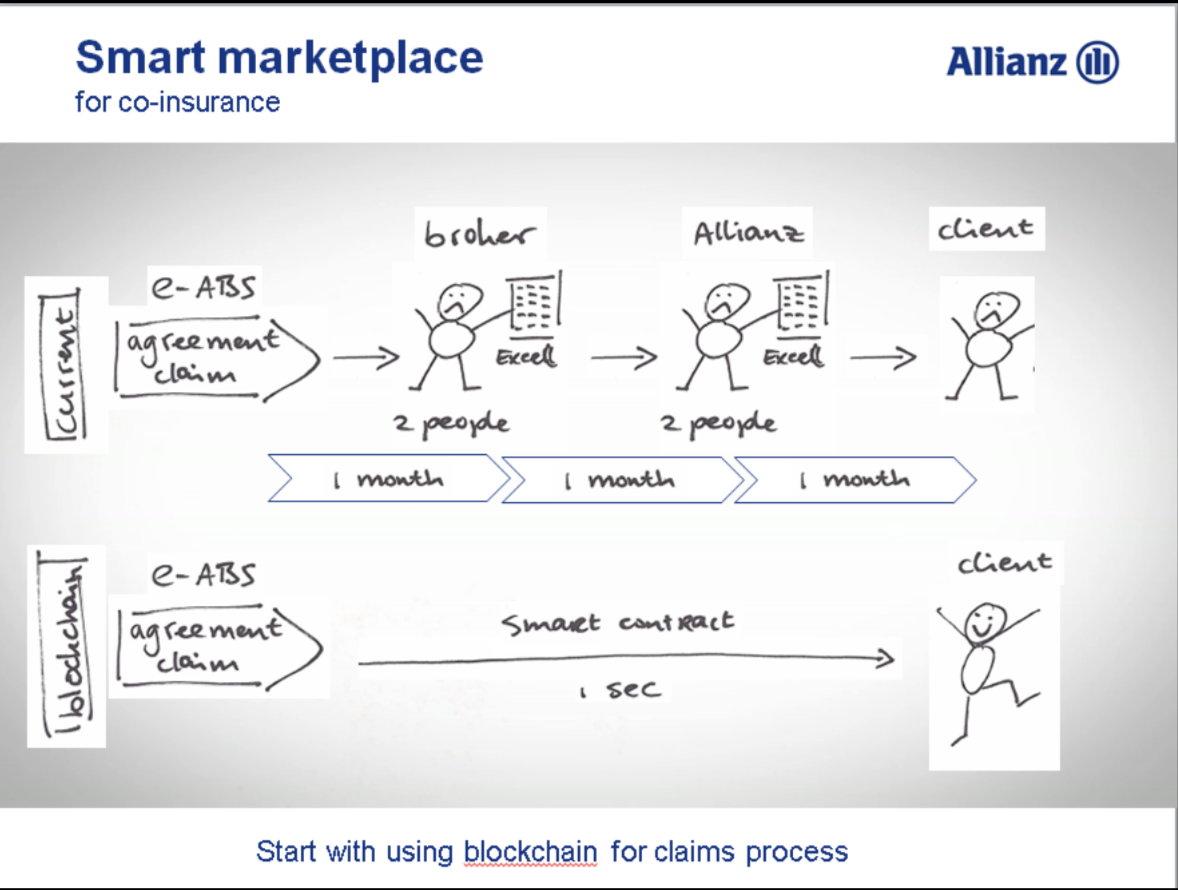
\includegraphics[scale=0.4]{images/allianz-blockchain}
        \caption{Usecase: co-insurance - Allianz}
        \label{fig:allianz-blockchain}
    \end{center}
\end{figure}

\newpage
\section{Onderzoek}
Op het moment van schrijven is het plan om onderzoek te doen naar de volgende hoofdvraag: ``\textit{Hoe is de blockchain technologie in te zetten om het claimproces van Allianz te automatiseren?}''\\
De volgende vragen komen aan bod:
\begin{itemize}
  \item Uit welke use cases, requirements en concerns bestaat het huidige proces van Allianz?
  \item Wat is de blockchain?
  \item Welke kansen \& knelpunten bestaan bij het toepassen van de blockchain?
  \item Hoe automatiseer je het huidige proces met de blockchain?
\end{itemize}
De huidige hoofd- en deelvragen kunnen nog gedurende het onderzoek veranderen. De laatste versie staan in het onderzoeksverslag.
\chapter{Projectgrenzen}
%Opschrijven wat je niet doet in je project geeft helderheid over wat je wel gaat doen. Hierdoor kun je ook voorkomen dat stakeholders tijdens het project met eisen komen die echt buiten de opdracht vallen. In deze paragraaf baken je je project dus af. In elk geval ga je hierbij in op hoe lang het project duurt, dus wanneer is het project klaar. Wat hoort inhoudelijk niet meer tot de opdracht? Bijvoorbeeld: ontwikkelen voor Windows, maar niet voor Linux; of wel een concept uitdenken, maar niet realiseren.
De afstudeeropdracht gaat van start op 5 februari 2018 en zal eindigen op 29 juni 2018. Het is de bedoeling dat ik gedurende de stageperiode aan de afstudeeropdracht en verslagen voor het afstuderen werk. Tijdens het onderzoek en analyse wordt enkel aandacht besteed aan onderwerpen die van belang zijn en een duidelijke toegevoegde waarde leveren aan het onderzoek en de proof of concept applicatie. Om de analyse en onderzoek correct en op tijd af te kunnen ronden wordt er aan alle onnodige zaken en informatie geen aandacht besteed.\par
Het project betreft alleen de use-case van Allianz en de mogelijkheden om het via de blockchain technologie op te lossen. Andere technologieën zijn uitgesloten, waarbij er wel binnen blockchain naar verschillende blockchain oplossingsrichtingen wordt gekeken. Er wordt tijdens dit afstudeerproject uiteindelijk maar één proof of concept opgeleverd en gepresenteerd aan de opdrachtgever. Enige nazorg na de stageperiode, of het hosten van software is niet van toepassing op dit project.

\section{Minimum Viable Product}
De Minimum Viable Product (MVP) voor het POC is als volgt voor dit project:
\begin{itemize}
  \item Broker: opstellen van co-insurance contracten (smart contract \footnote{https://en.wikipedia.org/wiki/Smart\_contract})
  \item Verzekerde: claim aanvragen
  \item Verzekeraar: claims goed of afkeuren
  \item Verzekeraar: automatische goed of
afkeuren op basis van business ruling
\end{itemize}
\chapter{Randvoorwaarden}
%Succesvol zijn gaat maar zelden ‘zomaar’. Bij randvoorwaarden geef je aan welke zaken geregeld moeten zijn zodat je zelf vlot door kunt werken. Denk bijvoorbeeld aan:
%- Ritme van de opleiding dicteert (denk hierbij bijvoorbeeld aan inleverdeadlines)
%- De opdracht gaat voor
%- Beschikbaarheid begeleider bedrijf. Is hij bijvoorbeeld op de juiste momenten beschikbaar
%voor het geven van feedback en het tijdig nemen van beslissingen?
%- Welke resources (b.v. soft- of hardware) moeten er zijn om te kunnen werken? Denk aan
%toegang tot systemen, ontwikkelsoftware, aanschaffen van benodigde licenties
%- Et cetera
Aan het afstudeerproject zijn enkele randvoorwaarden verbonden om een succesvol verloop te bevorderen. Deze randvoorwaarden zijn belangrijk voor de afbakening van het project. Hieronder staan de randvoorwaarden gegroepeerd weergegeven.\par

\section{m.b.t. afstudeerbedrijf}
\begin{itemize}
  \item Het project moet starten op 5 februari 2018;
  \item Het afstudeerbedrijf voorziet het projectlid van een werkruimte met daarin een laptop en internet.
  \item Het project moet op 29 juni 2018 afgerond zijn;
  \item De presentatie van het afstudeerproject moet gepland worden tussen 14 mei en 1 juni 2018;
  \item Het afstudeerproject wordt projectmatig en methodisch uitgevoerd.
  \item De stagiair besteedt 40 uur per week aan dit project;
  \item De uit te voeren activiteiten bestaan in principe alleen uit de afstudeer activiteiten die beschreven staan in het plan van aanpak;
  \item Het afstudeerproject wordt zelfstandig uitgevoerd en toont bekwaamheid competenties aan vanuit de courses in de studie;
  \item De stagair moet de bedrijfsbegeleider kunnen aanspreken in geval van onduidelijkheden;
  \item De bedrijfsbegeleider is aanwezig bij de bespreking van het concept van het projectplan met de docent begeleider;
  \item Aan het eind van het afstudeerproject vult de bedrijfsbegeleider een beoordelingsformulier over het functioneren van de afstudeerder in;
  \item De bedrijfsbegeleider is aanwezig is bij het mondelinge tentamen / de presentatie en verdediging van het afstudeerproject op school.
\end{itemize}

\newpage
\section{m.b.t. school}
\begin{itemize}
% \item Na elke twee weken wordt de voortgang gerapporteerd aan de school begeleider.
\item Geeft feedback op het projectplan (plan van aanpak);
\item Geeft feedback op de 80\% versie (reflectieverslag, onderzoeksverslag);
\item De schoolbegeleider bezoekt het stagebedrijf waarbij een gesprek plaatsvindt met de stagiair en de stagebegeleider;
\item Na het einde van de stageperiode vindt de afstudeerpresentatie plaats op school.
\end{itemize}
\chapter{Op te leveren producten en kwaliteitseisen}
%In dit hoofdstuk behandel je alle producten die je in hoofdstuk 5 beschreven hebt en moet opleveren, zoveel mogelijk in detail. Het gaat dan zowel om producten die je aan je opdrachtgever levert, als om de producten die de opleiding van je vraagt. Daarin verdeel je de resultaten die je moet opleveren een in kleinere (deel)producten. Zo kan het resultaat ‘een stuk werkende code’ bestaan uit een ontwerp, code, een testrapport en overdrachtsdocumentatie, etc.
De producten die ten behoeve van het afstudeeropdracht worden opgeleverd, dienen van voldoende kwaliteit te zijn. Om dit te garanderen zijn de volgende kwaliteitseisen beschreven in de onderstaande tabel.

\small
\begin{center}
 \begin{tabular}{|c c c c|} 
 
 \hline
 Product & Kwaliteitseisen & Activiteiten & Proceskwaliteit \\ [0.5ex] 
 \hline
 Plan van Aanpak & \makecell{
 - Voldoet aan ICA\\Controlekaart \cite{icaControl}\\
 - Voldoet aan ho-\\ofdstuk beschrijvingen\\ICA\cite{pvaTut}
 } & \cite{pvaTut} & \makecell{
 - Draft laten reviewen\\door minstens twee\\deskundigen
 } \\
 \hline

 \hline
 \makecell{
 Onderzoeksverslag\\
 } & \makecell{
 - Voldoet aan ICA\\Controlekaart \cite{icaControl}\\
 - Leidt af van Theo's\\ handleiding \cite{theoOnderzoek}
 } & \makecell{\cite{theoOnderzoek}\\\cite{icaOnderzoek}} & \makecell{
 - Draft laten reviewen\\door minstens twee\\deskundigen
 } \\
 \hline
 
 \hline
 Eindpresentatie & \makecell{
 - Voldoet aan ICA\\Controlekaart \cite{icaControl}
 } & \makecell{Opdrachtomschrijving,\\Process en resultaten,\\Conclussie} & \makecell{
 - Draft laten reviewen\\door minstens twee\\deskundigen
 } \\
 \hline
 
 \hline
 Reflectieverslag & \makecell{
 - Voldoet aan ICA\\Controlekaart \cite{icaControl}
 } & \makecell{
 Hoofdstukken: Inleiding,\\
 Opdrachtomschrijving\\
 Methode,\\
 Process en resultaten,\\
 Conclussie, Discussie\\
 Reflectie\\
 }& \makecell{
 - Draft laten reviewen\\door minstens twee\\deskundigen
 } \\
 \hline
 
 \hline
 Code & \makecell{
% -Unittests\\
 -Commentaar in het\\ Engels\\
 -Gebruik versiebeheer
 } & \makecell{
 -Schrijven code\\
 - SOLID \footnote{https://en.wikipedia.org/wiki/SOLID\_(object-oriented_design)}
% -Unit tests schrijven
 } & \makecell{
 - Statische code analyse\\
 - Refactoring
 } \\
 \hline
\end{tabular}
\end{center}
\end{small}

\newpage
\section{Competenties}
%De volgende stap is dat je kijkt of je met de producten die je moet opleveren je competenties voldoende kunt aantonen. Is dat niet het geval dan voeg je aan de lijst met ‘de producten voor de opleiding’ die onderdelen toe die nodig zijn om je opdracht ook voor de opleiding voldoende inhoud te geven. In elk geval staan de volgende zaken ook op die lijst: afstudeerverslag (inclusief reflectie en bijlagen), eindpresentatie, en voor semesterstudenten het onderzoeksrapport inclusief onderzoeksplan (voor profielers niet verplicht).
Om aan het einde en tijdens het afstudeerproject aan te kunnen tonen dat ik op aspirant hbo-niveau het project heb uitgevoerd. Behandeld dit hoofdstuk de competenties die ik tijdens het afstuderen ga aantonen. Deze competenties zijn een directe kopie uit de eindkwalificaties van de OER studie ICA handleiding 2017-2018 \cite{studiegids} en worden gekoppeld aan de eindproducten van dit project.

\subsection{SD-1: Software Requirements}
\textbf{Producten:} User stories, tickets, Proof of Concept \\
De student analyseert en specificeert de eisen aan een ICT-oplossing op basis van de gebruikersbehoeften op een gestructureerde en gestandaardiseerde manier. Valideert de opgestelde eisen.
Beheert (veranderende) eisen tijdens het softwareontwikkeltraject.

\subsection{SD-2: Software Design}
\textbf{Producten:} Onderzoeksverslag, Reflectieverslag \\
De student kan op basis van de requirements de interne structuur – de elementen en hun relaties - van een data- intensief en gedistribueerd softwaresysteem bepalen, zowel op top-level niveau (architectuur) als ook op gedetailleerd niveau (ontwerp).
\\
De student kan de gemaakte ontwerpkeuzes onderbouwen, past tijdens het ontwerpen standaard notaties en best practices uit het beroepenveld toe, en houdt in het ontwerp rekening met mogelijke onderhoudsvragen.

\subsection{SD-3: Software Architecture}
\textbf{Producten:} Onderzoeksverslag \\
De student kan op basis van de non-functional requirements de interne structuur op top-level niveau van een data-intensief en gedistribueerd softwaresysteem bepalen.
\\
De student kan de gemaakte architecturele keuzes onderbouwen en past tijdens het ontwerpen van de architectuur best practices uit het beroepenveld toe.

\subsection{SD-4: Software Construction}
\textbf{Producten:} Code, Proof of Concept \\
De student kan op basis van een ontwerp werkende en betekenisvolle data- intensieve en gedistribueerde software systemen realiseren, schrijft begrijpbare en hoogwaardige source code en past professionele tools en technieken toe om dit te bereiken, en kan in teamverband een volledig geïntegreerd en systeem opleveren, dat klaar is voor ingebruikname

\subsection{SD-5: Software Testing and Quality}
\textbf{Producten:} Code, Proof of Concept \\
De student kan aantonen dat het systeem aan de geïdentificeerde requirements voldoet en dat de opgeleverde producten, onder andere de source code, aan vooraf gedefinieerde kwaliteitscriteria voldoen.

\newpage
\subsection{SD-6: Software Engineering Process and Management}
\textbf{Producten: Plan van Aanpak, Onderzoeksverslag} \\
De student kan in een multidisciplinaire omgeving op grond van de gekozen ontwikkelmethodiek, passend bij de context en inhoud van de opdracht, een software-ontwikkeltraject projectmatig inrichten en uitvoeren, kiest geschikte methoden en technieken, past deze toe, en bewaakt de voortgang van het project door gebruik te maken van procesondersteunende tools.

\subsection{SD-7: Research}
\textbf{Producten:} Onderzoeksverslag, reflectieverslag \\
De student kan een probleem op het terrein van Software Development (bijvoorbeeld inzet van nieuwe technologieën) oplossen door een kleinschalig onderzoek uit te voeren op een systematische, methodisch verantwoorde wijze, en kan de conclusies daaruit onderbouwen en effectief communiceren.

\subsection{SD-8: Self support}
\textbf{Producten:} Plan van aanpak, Onderzoeksverslag, Eindpresentatie \\
De student kan als een beginnende professional zelfstandig een authentieke beroepsopdracht uitvoeren die leidt tot een of meer beroepsproducten en de uitvoering ervan verantwoorden.

\chapter{Ontwikkelmethoden}\label{chap:projectmethod}
%Nu je weet wat je gaat opleveren (producten en kwaliteit daarvan) en wat je daarvoor moet doen (overzicht activiteiten) met welke grenzen en randvoorwaarden, kun je bedenken wat de beste methode is om alles te realiseren. Heb je te maken met een ingevuld adviestraject dan ligt het voor de hand om eerst een onderzoek te doen en daarna met een advies te komen.
%Ben je bezig met het ontwerp van bijvoorbeeld een website of ga je een stuk software ontwikkelen, maak dan eerst een onderbouwde keuze tussen bijvoorbeeld waterval of incrementeel/iteratief. Daarbij spelen in elk geval de volgende overwegingen een rol:
%- In hoeverre kunnen de resultaten van het project snel en volledig worden beschreven?
%- Welke methoden hanteert het bedrijf en in hoeverre kun of moet je daar bij aansluiten? 
%Welke methoden ken je vanuit de opleiding?
%Wees hierbij wél kritisch: tijdens het afstuderen werk je bijvoorbeeld meestal in je eentje, en niet iedere methode (bijvoorbeeld Scrum bij het ontwikkelen van software) leent zich om individueel mee aan de slag te gaan. Soms is het handig om een methode daarop aan te passen. Dat kan, als je het maar goed onderbouwt en je daarbij baseert op betrouwbare bronnen. En als de methode is voorgeschreven: onderbouw waarom jij vindt dat deze methode passend is bij het soort project dat je moet gaan uitvoeren. Onderaan dit document vind je enkele suggesties voor literatuur over ontwikkelmethoden.
Gedurende het project wordt de agile softwareontwikkelmethode Kanban gehanteerd. Kanban is een lean fabricagemethoden (geïnspireerd op het Toyota Production System) en wordt voornamelijk gebruikt voor softwareontwikkeling en technologie gerelateerd werk. Kanban kan echter op elk werkgebied worden toegepast en kan zelfs worden gecombineerd met andere methoden of ontwikkelmethodieken zoals Scrum.\footnote{https://en.wikipedia.org/wiki/Kanban\_(development)}\par

Kanban lijkt vrij veel op Scrum, waar ik tijdens de loop van de studie veel in aanraking ben gekomen. Dit is gelijk ook de sterkste reden waarom er voor Kanban is gekozen. Kanban beperkt zich echter niet tot alleen Software development en past dus ook gelijk bij het onderdeel onderzoek in het project. Verder is er voor Kanban gekozen omdat het project niet in teamverband wordt uitgevoerd. Kanban in tegenstelling tot Scrum vereist niet de teamvergaderingen die normaal gesproken nodig zijn als het project in teamverband werd uitgevoerd (daily standups, retrospectives etc..). \par

Daarbij biedt deze iteratieve aanpak de mogelijkheid om het werk op te splitsen, in te schatten en prioriteiten te stellen in iteraties van 2 weken. Dit geeft de vereiste flexibiliteit om snel te kunnen schakelen bij aanpassingen. Gezien er onderzoek wordt uitgevoerd en er gebruik gemaakt wordt van experimentele software kan er gelijk begonnen worden aan een stuk onderzoek waarbij de bevindingen gelijk getest kunnen worden in het prototype (proof of concept).\par

Gedurende het project wordt er ook iteratief verbeterd. Na elke iteratie wordt er samen met de bedrijfsbegeleider gekeken naar het proces en mogelijke verbeteringen. Om deze feedback loop zo kort mogelijk te houden is er gekozen voor 2 weken iteraties en een Kanban WIP\footnote{https://kanbanize.com/kanban-resources/getting-started/what-is-wip/} limiet van één. Dit omdat het project niet in teamverband wordt uitgevoerd.
\chapter{Projectorganisatie en communicatie}
%Nu de verlangde resultaten en ontwikkelmethode bekend zijn kun je pas de projectorganisatie ( in 9.) en de planning (in 10.) behandelen. Dit hoofdstuk dat inzicht geeft in contactfrequenties tussen jou, de organisatie en de afstudeerdocent. Ga in elk geval in op:
%- Wie zijn je begeleiders (de opleiding en bedrijf)
%- Hoe vaak heb je contact met hen en waarover?
%- Wie is waarvoor verantwoordelijk
%- Wat zijn ieders –inclusief je eigen- contactgegevens?
De afstudeeropdracht wordt uitgevoerd door de stagiair waarbij ondersteuning wordt gegeven door de bedrijfsbegeleider. Daarnaast vindt er terugkoppeling plaats met de stagebegeleider die gezamenlijk samen met de assessor het project beoordeeld. De verdere projectorganisatie en context is beschreven in hoofdstuk \ref{chap:context}. De contactgegevens van de betrokkenen zijn hieronder weergegeven:\par
\paragraph{Stagair}~\\
Naam:		Calum Iain Munro\\
Telefoon:	06 835 426 80\\
E-mail:		CI.Munro@student.han.nl

\paragraph{Bedrijfsbegeleider \& Product owner}~\\
Naam:		Dani\"el Siahaya\\
Telefoon:	06 421 060 92\\
E-mail: 	Daniel@HeadFWD.com

\paragraph{Klant}~\\
Naam:		Arjan Zaal\\
Telefoon:	-\\
E-mail: 	arjan.zaal@allianz.nl

\paragraph{Stagebegeleider}~\\
Naam:		Misja Nabben\\
Telefoon:	06 553 720 69\\
E-mail:		Misja.Nabben@Han.nl

\paragraph{Assessor}~\\
Naam:		Rein Harle\\
Telefoon:	-\\
E-mail: 	Leon.bronckers@Han.nl

%\begin{sidewaysfigure}

\chapter{Planning}
%In dit hoofdstuk maak je een koppeling tussen de ontwikkelmethode en je activiteiten. Dit geef je weer in een GANTT-chart oftewel strokenplanning, waarin je je mijlpalen duidelijk weergeeft. Let op dat je ontwikkelmethode voldoende herkenbaar is in de planning.
Dit project wordt agile aangepakt. Meer hierover in het hoofdstuk ‘\nameref{chap:projectmethod}’. Deze aanpak probeert risico's te verminderen door software te ontwikkelen in korte, overzichtelijke perioden, die ‘iteraties’ genoemd worden. Het project is dus opgedeeld in iteraties van 2 weken, waarin in iedere iteratie bruikbaren producten worden opgeleverd.\par

Uit iedere iteratie wordt ook feedback ontvangen, waaruit het proces van het project zich continu verbeterd. Zodoende wordt er een stuk onderzocht en tegelijkertijd ook gewerkt aan een stuk prototype voor het proof of concept. Gedurende het project wordt er met de begeleider en input van de externe opdrachtgever besproken wat er in de iteratie wordt gedaan. Hieruit wordt vervolgens de todo swimming lane gevuld met werk voor die iteratie.

\section{GANTT-chart}

\begin{ganttchart}[vgrid, hgrid]{1}{21}
\gantttitle{februari}{4}
\gantttitle{maart}{4}
\gantttitle{april}{4}
\gantttitle{mei}{5}
\gantttitle{juni}{4}\\
\gantttitlelist{6,...,26}{1}\\
%Projectplan
\ganttgroup{Definitie Fase}{1}{6} \\
\ganttbar{Plan Van Aanpak}{1}{6} \\
\ganttmilestone{Concept projectplan}{3}\\
\ganttmilestone{Definitief projectplan}{6}\\
%Onderzoek
\ganttgroup{Analyse/Realisatie Fase}{5}{18} \\
\ganttbar{Iteratie 1}{5}{6} \\
\ganttbar{Iteratie 2}{7}{8} \\
\ganttbar{Iteratie 3}{9}{10} \\
\ganttbar{Iteratie 4}{11}{12} \\
\ganttbar{Iteratie 5}{13}{14} \\
\ganttbar{Iteratie 6}{15}{16} \\
\ganttbar{Iteratie 7}{17}{18} \\
%Afstudeerverslagen
\ganttgroup{Afronding Fase}{13}{20} \\
\ganttbar{Reflectieverslag}{13}{19} \\
\ganttbar{Presentatie}{20}{20} \\
\ganttmilestone{80\% versie}{15}\\
\ganttmilestone{Eindverslag}{19}\\
\ganttmilestone{Afstudeerpresentatie}{20}\\

\node [left] at ([yshift=-1.3cm]) {Week};
\end{ganttchart}
%\end{sidewaysfigure}

\newpage
\section{Opleverdata mijlpaalproducten}
In deze paragraaf zijn de uiterlijke opleverdata voor de mijlpaalproducten vermeld.

\small
\begin{center}
 \begin{tabular}{|c c|} 
 
 \hline
 Product & Datum \\ [0.5ex] 
 \hline
 Projectplan concept (Plan van Aanpak) & 23-02-2018 \\
 \hline
 Projectplan definitief (Plan van Aanpak) & 16-03-2018 \\
 \hline
 80\% versie (Onderzoeksverslag, POC, Reflectieverslag) & 14-05-2018 \\
 \hline
 Eindverslag (Onderzoeksverslag, POC, Reflectieverslag) & 11-06-2018 \\
 \hline
\end{tabular}
\end{center}
\end{small}

\chapter{Risico's}
%Dit hoofdstuk is een soort ‘final check’. De zaken die je kunt voorkomen door wijzigingen aan te brengen in de planning neem je alsnog op in je planning. Denk bijvoorbeeld aan voldoende overlegmomenten met je opdrachtgever. Alléén de risico’s die je niet vooraf kunt beïnvloeden neem je op in deze paragraaf. Een voorbeeld: als je weet dat je tijdens je project gaat verhuizen kun je in je planning opnemen op welke dagen je niet werkt. Afwezigheid door verhuizing is dus geen risico. Maar, als je afhankelijk bent van de levering van een server door een nieuwe leverancier, kan het anders zijn. Natuurlijk neem je eerst in de planning op dat je er nog een keer extra achter aan belt (dit noemen we een tegenmaatregel), maar je vraagt je ook af wat je gaat doen als het onverhoopt tóch misgaat (je uitwijkstrategie).
%Dit kun je weergeven in een tabel met als koppen: risico, kans (groot-middel-klein), impact (groot- middel-klein), tegenmaatregel, uitwijkstrategie.
In dit hoofdstuk worden de risico's tijdens het afstudeerproject benoemd en daar waar mogelijk opgevangen door een oplossing.\par

\section{Interne risico's}
Interne risico's vallen binnen de scope van het project of de verantwoordelijkheid van de projectorganisatie. In deze paragraaf worden de interne risico's benoemd.\par
\begin{itemize}
\item (Langdurige) ziekte van de stagiair. Dit wordt tijdig aangegeven aan de stagebegeleider en assessor, met verwachte datum van terugkomst. Daarnaast wordt dit risico gereduceerd door in de planning gebruik te maken van uitlooptijden.
\item Langdurige ziekte van de stagebegeleider. In dit geval dient direct een nieuwe assessor aangewezen te worden.
\item Langdurige ziekte van de bedrijfsbegeleider. In dit geval neemt een andere gekwalificeerde werknemer van HeadForward de begeleiding over. Dit risico wordt deels opgevangen door het feit dat er meerdere gekwalificeerde werknemers aanwezig zijn.
\item Een foutieve inschatting van de projectgrootte/projectduur. Het is mogelijk dat het project meer of minder tijd kost dan de uiteindelijke duur van het afstudeerproject. Mocht het project langer blijken te duren dan de totale afstudeertijd dan dient de opdracht in nauw overleg met de stagebegeleider en bedrijfsbegeleider dusdanig aangepast te worden dat deze in de beschikbare tijd kan worden afgerond. Mocht de opdracht voor het einde van het afstudeerproject voltooid zijn, dan verricht de stagiair in nauw overleg met de stagebegeleider en bedrijfsbegeleider aanvullende werkzaamheden.
\item Een gebrek aan begeleiding. De mogelijkheid bestaat dat de stagebegeleider en/of bedrijfsbegeleider onvoldoende tijd beschikbaar heeft voor het voldoende begeleiden van de stagiair. Dit kan afgevangen worden door begeleiding te zoeken bij andere werknemers.
\end{itemize}

\newpage
\section{Externe risico's}
Externe risico's liggen buiten de scope van het project en de projectorganisatie. In deze paragraaf worden de externe risico's benoemd.\par
\begin{itemize}
\item Onvolwassen technieken. De blockchain wordt momenteel nog amper tot niet gebruik in productieomgevingen. De documentatie en ondersteuning van sommige functies kan gebrekkig zijn waardoor het POC lastig te realiseren is. Hiervoor wordt er dan gezamenlijk met externe opdrachtgever gekeken naar alternatieven.
\item Verlies van gegevens door brand, diefstal en/of falende apparatuur. Door gebruik te maken van een versiebeheersysteem waarbij de software op meer dan één locatie opgeslagen is, wordt dit risico grotendeels afgedekt. Mochten er desondanks toch gegevens verloren gaan dan wordt hiervoor, in nauw overleg met de stagebegeleider, een oplossing gezocht.
\item Langdurige ziekte van de opdrachtgever. In dit geval neemt een andere gekwalificeerde werknemer van Allianz deze rol over. Dit risico wordt deels opgevangen door het feit dat er meerdere gekwalificeerde werknemers aanwezig zijn.
\end{itemize}



%%%%%%%%%%%%%%%%%%%%%%%%%%%%%%%%%%%%%%%%%%%%%%%%%%%%%%%%%%%%%%%%%%%%%%%%%%%%%%
%%
%% Bibliography:
%%
%\cleardoublepage
%\phantomsection
\addcontentsline{toc}{chapter}{Bibliografie}
\bibliography{thesis}

% %%%%%%%%%%%%%%%%%%%%%%%%%%%%%%%%%%%%%%%%%%%%%%%%%%%%%%%%%%%%%%%%%%%%%%%%%%%%%%%%
% %% Appendix:
% %%

\chapter{Bijlagen}
\appendix
\chapter{Competenties}\label{chap:competenties}
\subsection{SD-1: Software Requirements}
De student analyseert en specificeert de eisen aan een ICT-oplossing op basis van de gebruikersbehoeften op een gestructureerde en gestandaardiseerde manier. Valideert de opgestelde eisen.
Beheert (veranderende) eisen tijdens het softwareontwikkeltraject.

\subsection{SD-2: Software Design}
De student kan op basis van de requirements de interne structuur – de elementen en hun relaties - van een data- intensief en gedistribueerd softwaresysteem bepalen, zowel op top-level niveau (architectuur) als ook op gedetailleerd niveau (ontwerp).
\\
De student kan de gemaakte ontwerpkeuzes onderbouwen, past tijdens het ontwerpen standaard notaties en best practices uit het beroepenveld toe, en houdt in het ontwerp rekening met mogelijke onderhoudsvragen.

\subsection{SD-3: Software Architecture}
De student kan op basis van de non-functional requirements de interne structuur op top-level niveau van een data-intensief en gedistribueerd softwaresysteem bepalen.
\\
De student kan de gemaakte architecturele keuzes onderbouwen en past tijdens het ontwerpen van de architectuur best practices uit het beroepenveld toe.

\subsection{SD-4: Software Construction}
De student kan op basis van een ontwerp werkende en betekenisvolle data- intensieve en gedistribueerde software systemen realiseren, schrijft begrijpbare en hoogwaardige source code en past professionele tools en technieken toe om dit te bereiken, en kan in teamverband een volledig geïntegreerd en systeem opleveren, dat klaar is voor ingebruikname

\subsection{SD-5: Software Testing and Quality}
De student kan aantonen dat het systeem aan de geïdentificeerde requirements voldoet en dat de opgeleverde producten, onder andere de source code, aan vooraf gedefinieerde kwaliteitscriteria voldoen.

\subsection{SD-6: Software Engineering Process and Management}
De student kan in een multidisciplinaire omgeving op grond van de gekozen ontwikkelmethodiek, passend bij de context en inhoud van de opdracht, een software-ontwikkeltraject projectmatig inrichten en uitvoeren, kiest geschikte methoden en technieken, past deze toe, en bewaakt de voortgang van het project door gebruik te maken van procesondersteunende tools.

\subsection{SD-7: Research}
De student kan een probleem op het terrein van Software Development (bijvoorbeeld inzet van nieuwe technologieën) oplossen door een kleinschalig onderzoek uit te voeren op een systematische, methodisch verantwoorde wijze, en kan de conclusies daaruit onderbouwen en effectief communiceren.

\subsection{SD-8: Self support}
De student kan als een beginnende professional zelfstandig een authentieke beroepsopdracht uitvoeren die leidt tot een of meer beroepsproducten en de uitvoering ervan verantwoorden.



%%%%%%%%%%%%%%%%%%%%%%%%%%%%%%%%%%%%%%%%%%%%%%%%%%%%%%%%%%%%%%%%%%%%%%%%%%%%%%%%
%% Index:
%%
% \printthesisindex

\end{document}
